\documentclass[sigconf]{acmart}

\usepackage{graphicx}
\usepackage{hyperref}
\usepackage{todonotes}

\usepackage{endfloat}
\renewcommand{\efloatseparator}{\mbox{}} % no new page between figures

\usepackage{booktabs} % For formal tables

\settopmatter{printacmref=false} % Removes citation information below abstract
\renewcommand\footnotetextcopyrightpermission[1]{} % removes footnote with conference information in first column
\pagestyle{plain} % removes running headers

\newcommand{\TODO}[1]{\todo[inline]{#1}}
\newcommand{\DONE}[1]{DONE: \todo[inline,color=green!30]{#1}}

\usepackage{listings}
\usepackage{color}

\definecolor{dkgreen}{rgb}{0,0.6,0}
\definecolor{gray}{rgb}{0.5,0.5,0.5}
\definecolor{mauve}{rgb}{0.58,0,0.82}

\lstset{frame=tb,
  language=Python,
  aboveskip=3mm,
  belowskip=3mm,
  showstringspaces=false,
  columns=flexible,
  basicstyle={\small\ttfamily},
  numbers=none,
  numberstyle=\tiny\color{gray},
  keywordstyle=\color{blue},
  commentstyle=\color{dkgreen},
  stringstyle=\color{mauve},
  breaklines=true,
  breakatwhitespace=true,
  tabsize=3
}

\begin{document}
\title{Using Docker to Benchmark Virtual Machines}

\author{Ryan L. Irey, M.A.}
\orcid{1234-5678-9012}
\affiliation{%
  \institution{Indiana University}
  \streetaddress{107 S Indiana Ave}
  \city{Bloomington} 
  \state{Indiana} 
  \postcode{47405}
}
\email{rlirey@iu.edu}

% The default list of authors is too long for headers}
\renewcommand{\shortauthors}{R. Irey}

\begin{abstract}

VirtualBox, a commercially-available hypervisor maintained by Oracle, allows for the creation of lightweight, Docker-ready virtual machines running the Boot2Docker operating system. This project articulates a formula for the creation of a VirtualBox Boot2Docker machine, and demonstrates how the performance of the virtual machine can be benchmarked using popular utilities such as {\tt sysbench} and {\tt stress-ng}. The project will culminate with a simple Python application for collecting, persisting, and visualizing the benchmarked data.

\end{abstract}

\keywords{Benchmarking, Big Data, Boot2Docker, Docker, stress-ng, sysbench, VirtualBox, Virtual machine}

\maketitle

\section{Introduction}

Benchmarking is a common practice in which a system's architecture is measured under specific conditions that, ideally, are representative of the tasks performed on a day-to-day basis. From a theoretical standpoint, the history of computer benchmarking has endured spirited debate throughout the evolution of computing. As computer adoption continues to grow and computer applications further diversify, so too have benchmarking procedures and applications for measuring the capabilities of modern machinery evolved.

Docker is a platform that offers a variety of powerful tools, primarily for the containerization of applications and for creating computer clusters via their Swarm product. Moreover, the hypervisor VirtualBox allows for the creation of Boot2Docker virtual machines (VMs) which are VMs that are, for all intents and purposes, ''Docker-ready''. Building and deploying applications via containers is a relatively new concept, and so an understanding of appropriate benchmark procedures has yet to be well-defined. 

The scope of this manuscript is to describe a procedure for creating a Docker-ready virtual machine upon which a containerized benchmarking suite can be deployed. Within the benchmarking suite, a simple Python application collects and persists specific metrics from the benchmarking suite, culminating in a graphical visualization of the benchmarked data. 

\section{Benchmarking for Big Data}

The scope of big data analytics requires a tailored set of benchmarking tools, as the computational tasks that are representative of the day-to-day workload are likely very different from those leveraging consumer-level machines.

\begin{itemize}
  \item Workload evaluation
  \item Other things
  \item Other things
\end{itemize}

\section{System Architecture}

The host machine under study is a Macbook Pro manufactured by Apple, Inc. The machine is from the mid-2015 release cycle, and contains a 2.5 GHz Intel quad-core i7 processor and 16 GB of 1600 MHz DDR3 RAM. The host machine is running Docker Community Edition version 18.06.1 and Oracle VirtualBox version 5.2.18. 

\begin{itemize}
  \item VirtualBox + Boot2Docker VM
  \item Docker container w/ Benchmark tools
  \item Output graph
\end{itemize}

\section{Host Machine Setup}

\begin{itemize}
  \item Docker engine installation
  \item VirtualBox install
\end{itemize}

\section{Creating the Virtual Machine}

The host machine's Docker engine, coupled with the installation of the VirtualBox software, provides all of the tools necessary to create a virtual machine running the Boot2Docker operating system. To provision the virtual machine, enter the following command into the terminal:

\begin{lstlisting}
\$ docker-machine create --virtualbox-cpu-count "-1" --virtualbox-memory 1024 -d virtualbox vm
\end{lstlisting}



This code snippet will create a virtual machine using VirtualBox; the name of the virtual machine is given by the final argument, here, named ''vm''. The ''-1'' argument for --virtualbox-cpu-count allows the virtual machine to access all of the processing power of the host machine. Furthermore, specifying ''1024'' as the virtual memory allocation ensures that certain memory-related benchmark tasks, described below, are exercised appropriately with regard to the specified benchmark parameters.

\section{A Docker Container for Benchmarking}

In order to ensure the reproducibility of the benchmarking operations and their related scripts, the code for the benchmarking tasks is packaged as a Docker container. This has the added benefit of being very simple to deploy on the Boot2Docker operating system, on which the Docker engine is already installed.

\subsection{Benchmarks}

Five benchmark tasks were chosen to provide a look into the virtual machine's performance. As the workload of the machine has not been defined, the benchmarks are to be viewed as general purpose. From the five benchmark tasks, seven output metrics are captured; they are itemized as follows:

\subsubsection{Benchmark \#1: Prime number calculation}

Using the {\tt sysbench} cpu task, prime numbers are calculated between 0 and 100000 \cite{sysbench}. The metrics of interest derived from this task are (1) the number of events per second and (2) the average latency between calculations, given in milliseconds.

\subsubsection{Benchmark \#2: Random read/write}

Using the {\tt sysbench} fileio task, random read/write operations are performed in 16-kilobyte blocks up to a specified volume; in this instance, a volume cap of 2 gigabytes is used \cite{sysbench}. The metrics of interest are (3) the speed of read operations and (4) the speed of write operations, both in megabytes per second.

\subsubsection{Benchmark \#3: Matrix product}

Using the {\tt stress-ng} cpu task, this benchmark task calculates the matrix product of two 128x128 matrices comprised of double floating point values \cite{stressng}. The metric of interest is (5) the number of ''bogus'' operations per second.

\subsubsection{Benchmark \#4: HDD operations}

Using the {\tt stress-ng} hdd task, this benchmark task sequentially reads and writes temporary files for a duration of 30 seconds \cite{stressng}. Specifically, multiple buffer I/O's are used, and 16 files are read/written at a time. The metric of interest is (6) the number of ''bogus'' operations per second.

\subsubsection{Benchmark \#5: Memory Thrashing}

Using the {\tt stress-ng} memthrash task, this benchmark task iterates over a spate of memory thrashing stressor methods wherein each stressor starts at least one 16MB buffer thread per CPU for a duration of 30 seconds  \cite{stressng}. The metric of interest is (7) the number of ''bogus'' operations per second.

\subsection{Python application}

The main purposes of the Python application are to extract the benchmark data from the log files put out by each benchmark task, save any repeated measurements to a master table, and to produce visualizations of the benchmark data. The data extraction is accomplished by taking in each log file, converting the data to strings, parsing the strings into a list, and then selecting the appropriate string from the list. For example, the data for Benchmark \#1 is extracted as such:

\begin{lstlisting}
cpu = pd.read_csv("./cpu.txt", error_bad_lines = False)
eps = (cpu[list(cpu.columns)[0]].iloc[8]).split(" ")
eps = [eps[i] for i in range(len(eps)) if len(eps[i]) > 0][-1]
eps = float(eps)
\end{lstlisting}

Data from each benchmarking task is extracted in a similar manner and saved to a master table for persistence.

\subsection{Containerization with Docker}

\begin{lstlisting}
FROM ubuntu:18.04
LABEL maintainer="rlirey@iu.edu"

RUN apt-get update --fix-missing
RUN apt-get upgrade -y
RUN apt-get install sudo -y
RUN sudo apt-get install stress-ng -y
RUN sudo apt-get install sysbench -y
RUN sudo apt-get install -y tzdata
RUN sudo apt-get install -y python3-tk python3-setuptools python3-pip
RUN mkdir -p /myapp

WORKDIR /myapp

COPY . .

RUN pip3 install -r requirements.txt

CMD ["/bin/bash"]
\end{lstlisting}

The Dockerfile specifies the configuration of the different layers comprising the Docker container. Here, the container is built on a base Ubuntu image. The Dockerfile subsequently handles the updating of some Ubuntu utilities, and proceeds to install the benchmark tools comprising the suite under study. Next, the relevant bash and python script files are copied. Finally, the Python package requirements are installed via {tt\ pip}.

\subsection{Executing the benchmark suite}
The Docker container is initialized by running the following code snippet. Explicitly naming the container will alleviate some of the cumbersome nature of viewing the benchmark plot.

\begin{lstlisting}
\$ docker run -it --name=i523proj rlirey/i523-project
\end{lstlisting}

With the aforementioned Docker container up and running, a bash shell is the first point of contact the user has with the container. Each iteration of the benchmark suite requires the execution of the following code snippet:

\begin{lstlisting}
\$ python3 ./code/i523-proj.py
\end{lstlisting}

After the first execution of the benchmark suite, the user will notice that a benchGraph.png file is created in the directory. Subsequent executions of the benchmark suite will update the image file with data points from each execution.

\section{Visualizing Benchmark Data}

One product of the Python program is a Pandas data frame, on which the matplotlib library can easily be called for visualization purposes. Ultimately, the output of the Python program is a PNG file that plots each of the five benchmark measures in a single figure. For example, after five iterations of data collection, a visualization akin to that in Figure \ref{f:plotMBP} is produced. The data in Figure \ref{f:plotMBP} is that observed over six iterations of the benchmark suite on the baseline host machine, the Apple Macbook Pro.

\begin{figure}[!ht]
  \centering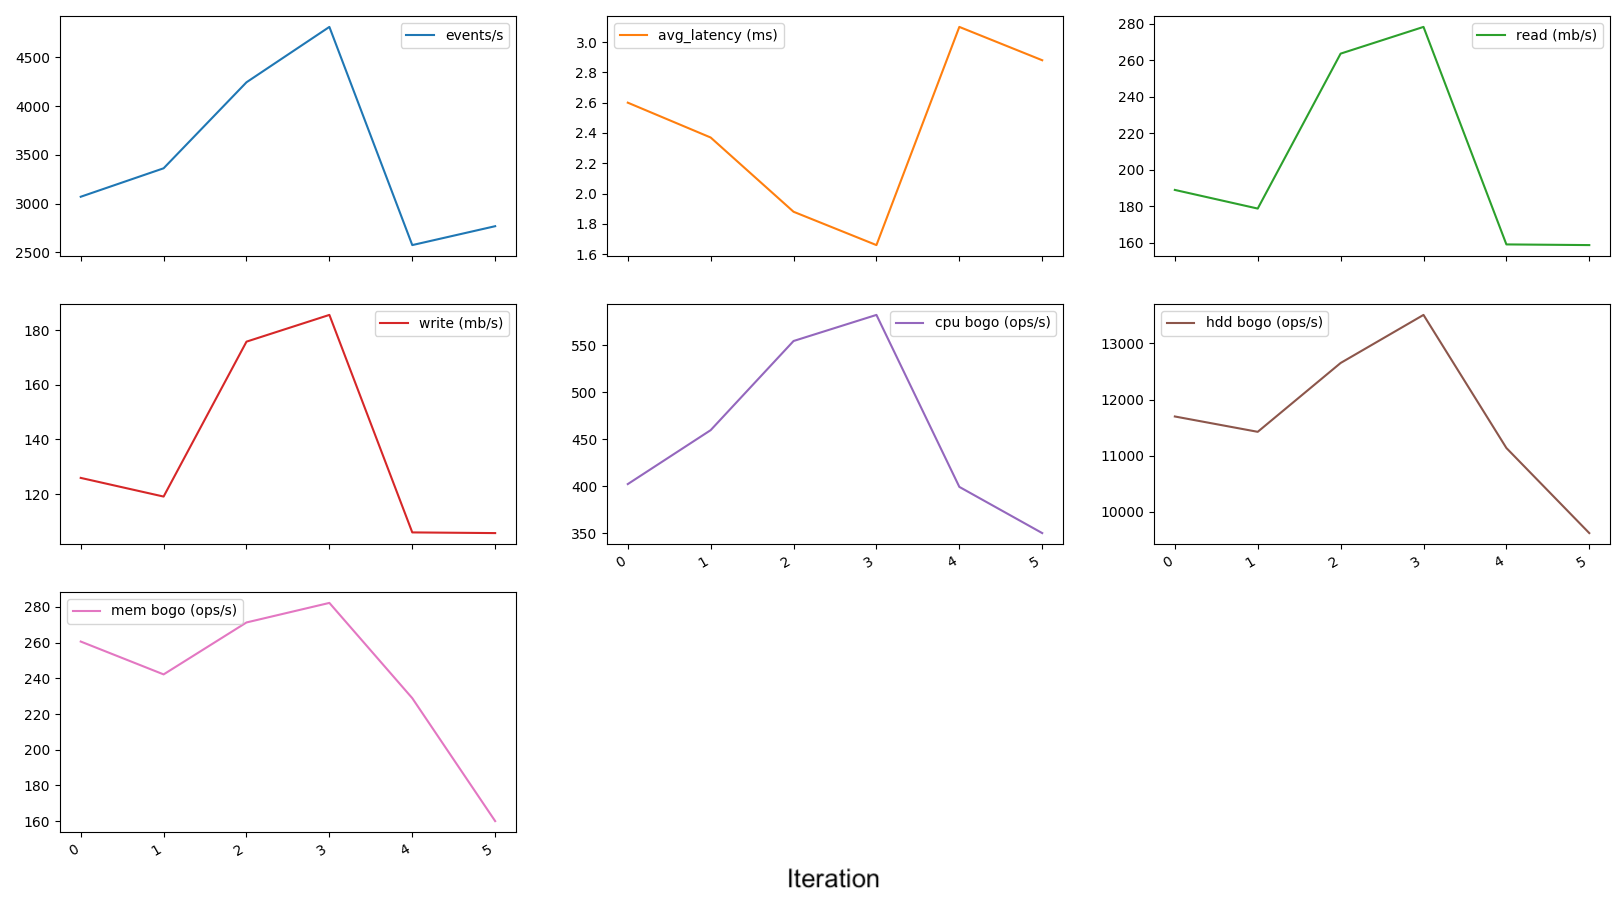
\includegraphics[width=\columnwidth]{images/samplePlot.png}
  \caption{A visualization of the benchmarking data after six iterations on the baseline host machine (Apple Macbook Pro).}\label{f:plotMBP}
\end{figure}

\section{A cloud-based comparison}

\subsection{Preparing the cloud environment}

Setting up a cloud-based computational environment is a relatively straight-forward process, the details of which are beyond the scope of this manuscript. It is assumed that the reader is familiar with the initialization process of the Amazon Web Services (AWS) EC2 platform, which allows for the creation of cloud-based computational environments of various hardware and software configurations and complexities. Here, for comparison with the baseline host machine, an AWS Ubuntu Server is deployed, accessible via {\tt ssh} in the bash shell. 

\begin{lstlisting}
\$ ssh -i </path/to/key> \ ubuntu@<server_address>.amazonaws.com
\end{lstlisting}

The AWS server runs Ubuntu Server version 18.04, and contains 96 processing cores and 384 GB of RAM with a 25 Gigabit network interface. This configuration was selected for its stark differences in system architecture when compared with the baseline host machine. The only prerequisite to executing the benchmark suite on the AWS Ubuntu server is to install the Docker engine via the command line. The details of Docker installation via the command line are easy to follow and provided in Docker's documentation library; thus, they will not be detailed here.

\subsection{Executing the benchmark suite}

With the Docker engine successfully installed on the AWS Ubuntu server, the execution of the containerized benchmark suite is identical to that on the baseline host machine:

\begin{lstlisting}
\$ docker run -it --name=i523proj rlirey/i523-project
\end{lstlisting}

Recall that executing the container results in a command line interface from within the container. The user simply follows the same steps as outlined above for the baseline host machine:

\begin{lstlisting}
\$ python3 ./code/i523-proj.py
\end{lstlisting}

Running the above code snippet multiple times will result in the population of a data for each iteration, as expected.

\subsection{Extraction of results}
After running six iterations of the containerized benchmark tools, the visualization of the outcomes is ready for extraction. Recall that the image extraction is a two-step process. First, from the Ubuntu server's command line, the image is copied out of the Docker container via Docker's {\tt cp} (copy) command:

\begin{lstlisting}
sudo docker cp i523proj:/myapp/benchGraph.png .
\end{lstlisting}

With the graph image now copied out of the container, the file can now be copied from the Ubuntu server to the final destination, the host machine, via the {tt\ scp} (secure copy) command: 

\begin{lstlisting}
sudo scp -i </path/to/key> \ ubuntu@<server_address>.amazonaws.com:~/benchGraph.png .
\end{lstlisting}

Now that the graph image file is copied to the host machine, it can be opened and examined. Figure \ref{f:plotAWS} displays such a visualization, as obtained by the AWS Ubuntu server.

\begin{figure}[!ht]
  \centering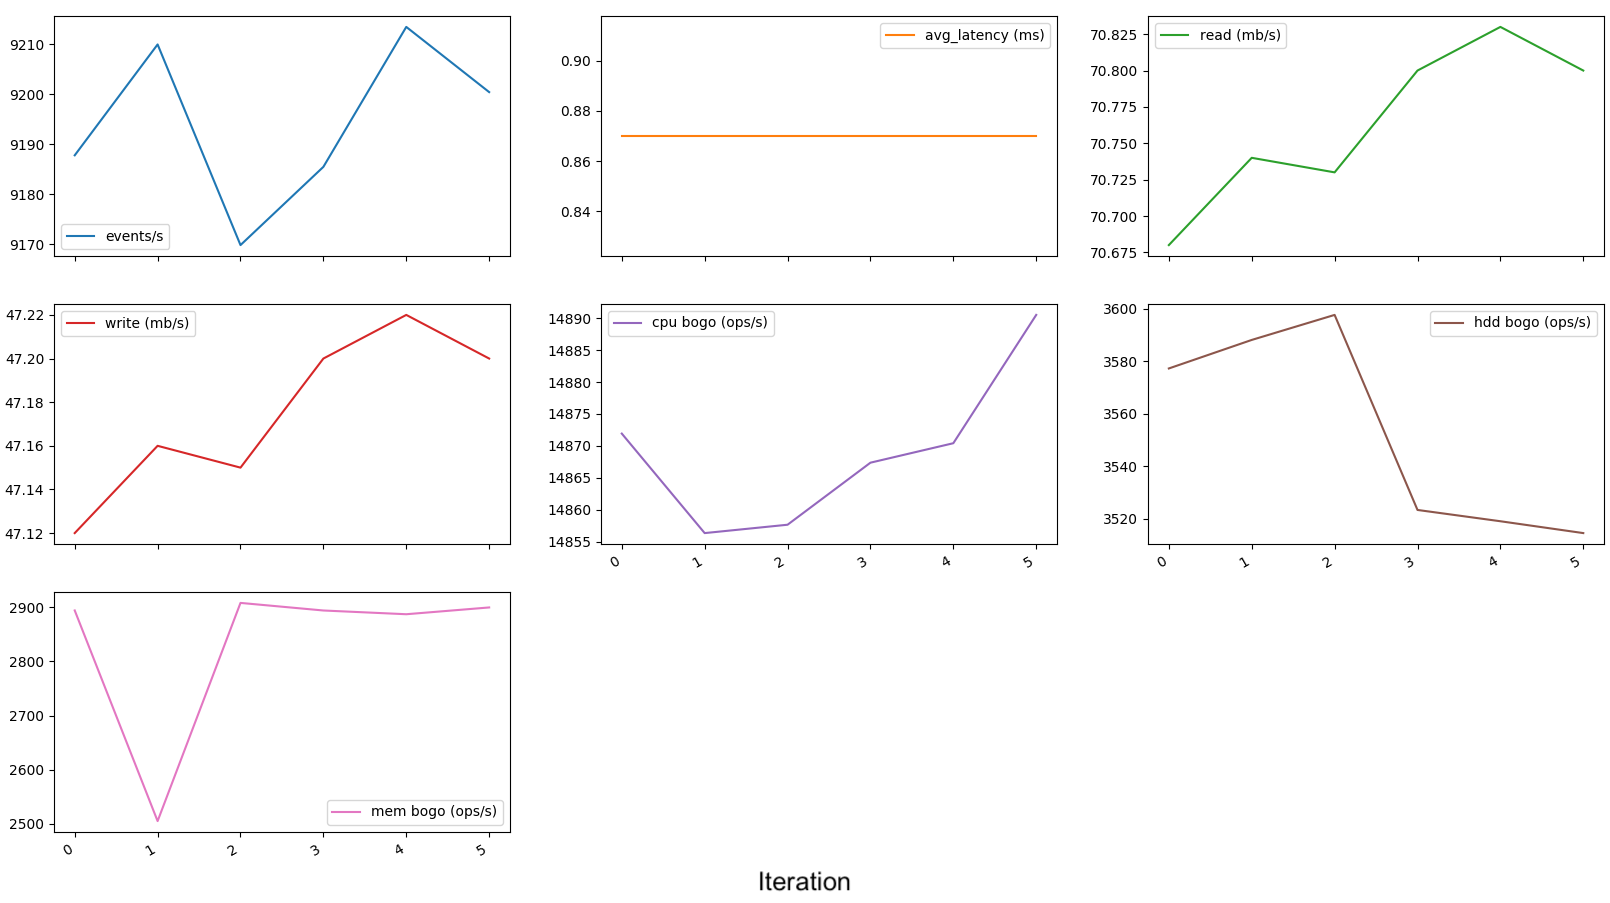
\includegraphics[width=\columnwidth]{images/benchGraph_AWS.png}
  \caption{A visualization of the benchmarking data after six iterations on the cloud-based comparison machine (Amazon Web Services Ubuntu Server).}\label{f:plotAWS}
\end{figure}

\subsection{Comparison of findings}

A close examination of \ref{f:plotMBP} and \ref{f:plotAWS} reveals several important observations.

\subsubsection{Benchmark \#1 and \#2: Prime number calculation and latency}

The number of prime number calculation events per second spans a wide range on the baseline host machine, varying by around 2000 events in subsequent iterations. On the AWS Ubuntu server, not only is the raw number of events per second almost double that of the baseline host machine, the variance in measurements across iterations is much tighter than that of the baseline host machine. The average latency between calculations on the host machine varies slightly between approximately 1.5 and 3.0 ms, whereas the latency between calculations on the AWS Ubuntu server is much lower, approximately 0.87 ms, staying relatively constant over subsequent iterations.

\subsubsection{Benchmark \#3 and \#4: Random read/write}

On the baseline host machine, whose hard disk storage is soldered directly to the logic board, the read and write speeds follow a very similar trajectory over the course of six iterations, spiking with read speeds approaching 200 mb/s and write speeds approaching 180 mb/s. Since the AWS Ubuntu server has a limited amount of network-attached EBS storage, the read and write speeds are considerably slower than that of the baseline host machine, although the trajectory of the read/write speeds generally increases over the course of six iterations.

\subsubsection{Benchmark \#5: Matrix product}

Matrix product calculation operations for the baseline host machine follows a concave trajectory, varying by almost 100 operations per second over subsequent iterations. Conversely, matrix product calculation operations for the AWS follows a convex trajectory, running nearly three times the number of operations per second compared to the baseline host machine. This is likely attributed to the much greater count of processing cores found in the system configuration of the AWS Ubuntu server.

\subsubsection{Benchmark \#6: HDD operations}

The trajectory of the HDD operations across iterations is similar between the baseline host machine and the AWS Ubuntu server. However, the raw number of operations per second is around 60\% fewer for the AWS Ubuntu server, likely due to its hard disk storage configuration as a network-attached volume.

\subsubsection{Benchmark \#7: Memory Thrashing}

Memory thrashing operations on the baseline host machine stay relatively constant over the course of several iterations, before plummeting by nearly 100 operations per second in subsequent iterations. The AWS Ubuntu server, however, maintains a much greater number of operations per second over the course of several iterations (with the exception of one obvious anomalous measurement). These differences can be attributed to the stark differences in RAM between the two system architectures.

\section{Limitations}

The Python program produces a graphical output of the benchmark tests called ''benchGraph.png''. However, one severe limitation of this project is the ability to easily open the image for inspection. Efforts to connect the Docker container to the host machine's X11 service were not successful, and so useful command line image viewers such as {\tt feh} are not utilized here. As a workaround, a shell script called ''copyImage.sh'' aids in the transfer of the ''benchGraph.png'' in two stages. As described above, the image is first transferred from inside the Docker container to the VirtualBox virtual machine. The image is then transferred from the VirtualBox virtual machine to the host machine, where the image can be successfully opened and inspected. 

\section{Extensions}

\subsection{Use with clusters/Docker swarm}

\begin{itemize}
  \item Think of
  \item some stuff
  \item to write here
\end{itemize}

\subsection{Practical applications for Big Data}

\begin{itemize}
  \item Think of
  \item some stuff
  \item to write here
\end{itemize}

\section{Conclusion}
The scope of big data analytics requires a tailored set of benchmarking tools, as the computational tasks that are representative of the day-to-day workload are likely very different from those leveraging consumer-level machines. This project describes a procedure for creating a Docker-ready virtual machine within which a containerized benchmarking suite is deployed, allowing for the collection, persistence, and visualization of benchmarked data. This framework can easily be extended to specific big data applications by tailoring the specific benchmarking tests, estimated workload, and other specific tasks for containerized deployment on local hosts, virtual machines, or cloud-based systems.

\begin{acks}

The author would like to thank Dr. Gregor von Laszewski and all teaching assistants of INFO-I523 for their thoughtful comments and guidance on previous versions of this manuscript.

\end{acks}

\bibliographystyle{ACM-Reference-Format}
\bibliography{report} 





\appendix

We include an appendix with common issues that we see when students submit papers. One particular important issue is not to use the underscore in bibtex labels. Sharelatex allows this, but the proceedings script we have does not allow this.

When you submit the paper you need to address each of the items in the issues.tex file and verify that you have done them. Please do this only at the end once you have finished writing the paper. To do this change TODO with DONE. However if you check something on with DONE, but we find you actually have not executed it correcty, you will receive point deductions. Thus it is important to do this correctly and not just 5 minutes before the deadline. It is better to do a late
submission than doing the check in haste. 

\section{Issues}

\DONE{Example of done item: Once you fix an item, change TODO to DONE}

\subsection{Assignment Submission Issues}

    \TODO{Do not make changes to your paper during grading, when your repository should be frozen.}

\subsection{Uncaught Bibliography Errors}

    \TODO{Missing bibliography file generated by JabRef}

\subsection{Formatting}

    \TODO{Incorrect number of keywords or HID and i523 not included in the keywords}

\subsection{Writing Errors}

    \TODO{Errors in title, e.g. capitalization}

\subsection{Citation Issues and Plagiarism}

    \TODO{It is your responsibility to make sure no plagiarism occurs. The instructions and resources were given in the class}

\subsection{Character Errors}

    \TODO{Erroneous use of quotation marks, i.e. use ``quotes'' , instead of " "}

\subsection{Structural Issues}

    \TODO{Acknowledgement section missing}

\subsection{Details about the Figures and Tables}

    \TODO{Capitalization errors in referring to captions, e.g. Figure 1, Table 2}

\end{document}